\documentclass{beamer}

% Required packages
\usepackage{tikz}
\usepackage{listings}
\usepackage{xcolor}

% Define custom colors
\definecolor{ds9blue}{RGB}{25,25,112}
\definecolor{ds9gold}{RGB}{218,165,32}
\definecolor{ds9grey}{RGB}{105,105,105}
\definecolor{ds9red}{RGB}{178,34,34}

% Theme configuration
\usetheme{Madrid}
\usecolortheme{whale}
\setbeamercolor{structure}{fg=ds9blue}
\setbeamercolor{alerted text}{fg=ds9red}
\setbeamercolor{example text}{fg=ds9gold}

% Title page configuration
\title[Intro to Arrays]{Introduction to Arrays in C++}
\subtitle{From Variables to Collections}
\author[Mr. Gullo]{Mr. Gullo}
\date[\today]{\today}

% Configure code listings
\lstset{
    language=C++,
    basicstyle=\ttfamily\small,
    keywordstyle=\color{ds9blue},
    stringstyle=\color{ds9gold},
    commentstyle=\color{ds9grey},
    numbers=left,
    numberstyle=\tiny,
    numbersep=5pt,
    frame=single,
    breaklines=true
}

\begin{document}

% Title page
\begin{frame}
    \titlepage
\end{frame}

% Learning objectives
\begin{frame}{Learning Objectives}
    \begin{block}{After this lesson, you will be able to:}
        \begin{itemize}
            \item Understand arrays as contiguous memory structures
            \item Declare and initialize arrays effectively
            \item Perform common array operations
            \item Implement array-based solutions
            \item Avoid common array pitfalls
        \end{itemize}
    \end{block}
\end{frame}

% Memory Layout
\begin{frame}{Array Memory Layout}
    \begin{columns}[T]
        \begin{column}{0.5\textwidth}
            \begin{itemize}
                \item Contiguous memory allocation
                \item Each element occupies fixed space
                \item Direct access via index
            \end{itemize}
        \end{column}
        \begin{column}{0.5\textwidth}
            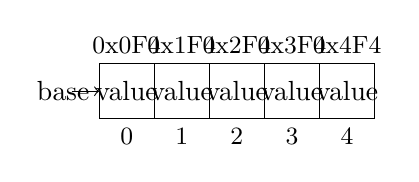
\begin{tikzpicture}[scale=0.7]
                % Memory blocks
                \foreach \x in {0,1,2,3,4} {
                    \draw (\x,0) rectangle (\x+1,1);
                    \node at (\x+0.5,0.5) {value};
                    \node[below] at (\x+0.5,0) {\small\x};
                    \node[above] at (\x+0.5,1) {\small 0x\x F4};
                }
                % Memory address arrow
                \draw[->] (-0.5,0.5) -- (0,0.5) node[left] {base};
            \end{tikzpicture}
        \end{column}
    \end{columns}
\end{frame}

% Array Declaration and Initialization
\begin{frame}[fragile]{Array Creation}
    \begin{block}{Declaration Methods}
        \begin{lstlisting}
// Method 1: Declaration with size
int temperatures[7];  // Uninitialized array

// Method 2: Declaration with initialization
int scores[5] = {95, 88, 76, 90, 85};

// Method 3: Size inference
int fibonacci[] = {1, 1, 2, 3, 5, 8, 13};

// Method 4: Partial initialization
int values[5] = {0};  // Sets all to 0
        \end{lstlisting}
    \end{block}
\end{frame}

% Array Access and Modification
\begin{frame}[fragile]{Working with Arrays}
    \begin{lstlisting}
int numbers[] = {10, 20, 30, 40, 50};

// Reading elements
int first = numbers[0];    // Get first (10)
int last = numbers[4];     // Get last (50)

// Modifying elements
numbers[2] = 35;           // Change middle element
numbers[4] += 5;           // Increment last element

// Common mistake: bounds
// numbers[5] = 60;        // ERROR: Out of bounds!
    \end{lstlisting}
\end{frame}

% Array Traversal
\begin{frame}[fragile]{Array Traversal Patterns}
    \begin{lstlisting}
int data[] = {1, 2, 3, 4, 5};
int size = 5;

// Forward traversal
for(int i = 0; i < size; i++) {
    cout << data[i] << " ";
}

// Reverse traversal
for(int i = size - 1; i >= 0; i--) {
    cout << data[i] << " ";
}

// Skip pattern (every second element)
for(int i = 0; i < size; i += 2) {
    cout << data[i] << " ";
}
    \end{lstlisting}
\end{frame}

% Practical Example 1
\begin{frame}[fragile]{Example: Temperature Analysis}
    \begin{lstlisting}
// Find average daily temperature
double getAverageTemp(int temps[], int days) {
    double sum = 0;
    for(int i = 0; i < days; i++) {
        sum += temps[i];
    }
    return sum / days;
}

// Find temperature range
void getTempRange(int temps[], int days, 
                 int& min, int& max) {
    min = max = temps[0];
    for(int i = 1; i < days; i++) {
        if(temps[i] < min) min = temps[i];
        if(temps[i] > max) max = temps[i];
    }
}
    \end{lstlisting}
\end{frame}

% Practical Example 2
\begin{frame}[fragile]{Example: Data Processing}
    \begin{lstlisting}
// Count occurrences in an array
int countValue(int arr[], int size, int target) {
    int count = 0;
    for(int i = 0; i < size; i++) {
        if(arr[i] == target) count++;
    }
    return count;
}

// Check if array is sorted
bool isSorted(int arr[], int size) {
    for(int i = 1; i < size; i++) {
        if(arr[i] < arr[i-1]) return false;
    }
    return true;
}
    \end{lstlisting}
\end{frame}

% Common Errors and Best Practices
\begin{frame}{Array Best Practices}
    \begin{alertblock}{Common Pitfalls}
        \begin{itemize}
            \item Array bounds violations
            \item Off-by-one errors in loops
            \item Uninitialized array access
            \item Forgetting array size limits
        \end{itemize}
    \end{alertblock}
    
    \begin{block}{Best Practices}
        \begin{itemize}
            \item Always track array size
            \item Initialize arrays when declared
            \item Use bounds checking
            \item Consider using std::array when possible
        \end{itemize}
    \end{block}
\end{frame}

% Summary
\begin{frame}{Key Takeaways}
    \begin{columns}[T]
        \begin{column}{0.5\textwidth}
            \begin{block}{Core Concepts}
                \begin{itemize}
                    \item Contiguous memory
                    \item Zero-based indexing
                    \item Fixed size
                    \item Type consistency
                \end{itemize}
            \end{block}
        \end{column}
        \begin{column}{0.5\textwidth}
            \begin{block}{Operations}
                \begin{itemize}
                    \item Element access
                    \item Array traversal
                    \item Data processing
                    \item Bounds checking
                \end{itemize}
            \end{block}
        \end{column}
    \end{columns}
\end{frame}

\end{document}